
\section{Traffic Engineering}


Network traffic engineering is an old discipline in the telecommunication industry and has evolved with certain specificities for different networks types. This overview focus on the issues and techniques related to Internet and IP networks Traffic Engineering, yet many of these concepts are valid for other network contexts.

\subsection{Definition and problem description}
Traffic engineering is the discipline concerned with the performance evaluation  and optimization of  networks.  This aspect of network engineering applies technology and scientific principles to measure, model and control the traffic.  \cite {RFC3272}.  

The main objective behind this intervention is to enhance the network efficiency, as it is perceived  from both  traffic and  resources views. The first one is usually referred to as traffic oriented, and is concerned with the enhancement of the quality of service (QoS) parameters as seen by traffic flows. Including : minimization of delay, minimization of packet loss and maximization of the throughput. In particular, the aim of this project as mentioned above, will be the minimization of loss rate as the main objective of our traffic engineering protocol.

Meanwhile, the second category of policies said resource oriented,  deals instead with the aspect related to the optimization of the resource utilization. In fact, having some subsets of the network being over-utilized while others are underutilized is an indication of a network not being used optimally. Maximum path utilization is usually used in this context as the principle evaluation measurement for network performance. TEXCP (see 2.1.4), the protocol that we'll be comparing with the results of our own architecture is an example of such approach. 

But the question that many might ask is how much TE could enhance the network efficiency? And does it really bring a significant added value? Doubts about TE utility usually use the tremendous increase of equipments capacity to promote that the demand on the network could be answered by simply putting more capacity on the network and that it won't significantly increase the network operator bill since marginals cost are converging to effectively zero. However, this vision of the Internet is simplistic. Internet has evolved from a simple network for the research community to a sophisticated communication infrastructure that provides a rich panel of services. The new users of Internet can't settle any more for the range of best  effort services that the network offered initially. Network operators need to make sure that their customers are receiving the service they are requiring, and that they are able to differentiate the charging according to  these requirements. Moreover, the near deployment of  optical fibers and the increase of users expectation will mean that there will be more demand on the operator core network. The efficiency boost that TE could bring will help the operators to keep their margin. This is especially crucial in open market where fierce competition is taking place. The global context of convergence is taking down the incomes of classical operators, and the only way to keep a profit margin is by reducing cost and take the most from network their key asset. This is what Traffic Engineering attempts to achieve.

\subsection{Basic Concepts}

\subparagraph{TE as a controllability problem }:
\\Independently from the optimization policy approach, a set of control tools and mechanisms are usually invoked in order to accomplish this policy. These control actions could be divided in three categories: 

Acting on {\bf traffic management} parameters is used police aggressive users or to support services with differentiated Quality of Service. This could be achieved by using techniques like queue management, differentiated scheduling and traffic policing and shaping.

Acting on {\bf resources attributes and constraints} that include controlling link bandwidth, buffers etc.
 
Modification of {\bf routing parameters} to control how traffic steers within the network. 

\subparagraph{Routing and Traffic Engineering }:
\\This last category is particularly important in this project since it is primarily involved in taking advantage of path diversity within a network. The Internet hourglass implies that network should be kept simple with routing is the key provided function. The routing process involves core network nodes or routers to choose the path over which to send packets. One of the Internet design principle  for the network is that it should be kept plane and without any central nodes that might introduce  vulnerability. This means that routing protocol have as a requirement allowing the routers to take local decisions while ensuring consistency and packet being delivered to their destinations. Routing protocol like RIP and OSPF succeed in this purpose. However, the topology driven nature of these protocols implies that they optimize the path choice of each destination independently without considering the traffic demand on the network.  A solution that allows to go around these limitations could be achieved solution by manipulating configuration parameters of the previous routing protocols to enhance network performance.  In particular, by having an estimation of the traffic demand on the network, network management could choose the link weights  used by OSPF for example, on a way that results in an optimized distribution of traffic over the network could be achieved. In \cite{fortz00} an iterative algorithm is describe to optimize the network utilization by adjusting the weight through the use of heuristic mechanisms. This solution presents many advantages like compatibility with existing routing protocols and stability. In the other hand weight update frequency should be kept low since during updates routing consistency is not ensured.

\subparagraph{Traffic Engineering in MPLS networks}:
\\Routing restrictions are one of the difficulties encountered with traditional IP networks. MPLS  Multi Protocol Label Switching answers some of them by using a connection-oriented switching mechanism:  At the edge of an MPLS domain, the ingress LSR (Label Switching Router) adds a header to the packet and forwards it (see figure \ref{fig:mpls-header}). The label field in the header indicates to which FEC (Forwarding Equivalence Class) the packet belongs so core LSRs knows how to process it (in case of differentiated service) and where to send it next. 

\begin{figure}[h]
 \begin{center}

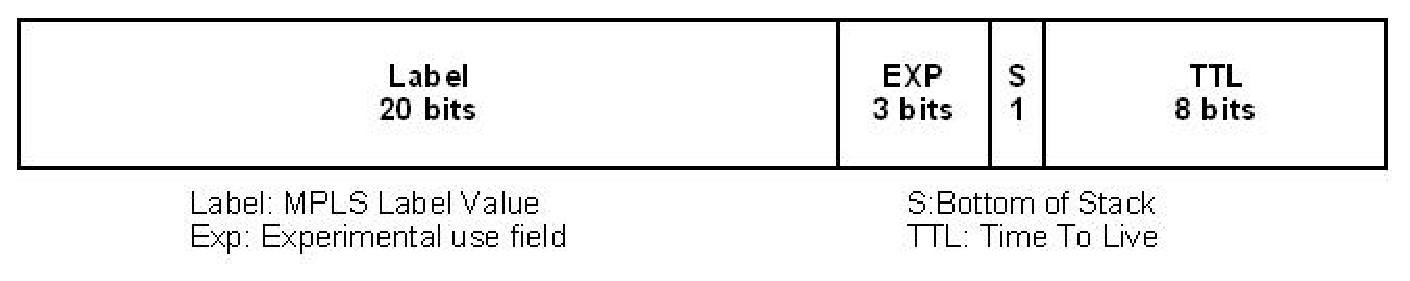
\epsfig{file=img/sec-2-1/1, width=4.5in}
\caption{
   The format of the MPLS header.

    \label{fig:mpls-header}
}
\end{center}
\end{figure}

MPLS allows the network management to provision tunnels within the network by configuring the core LSR. Edge LSRs are also configured to how they should assigned incoming traffic to these tunnels. This open the way for new Traffic Engineering capabilities. After gathering information about the traffic, the network management configures tunnels and assigns the traffic to them in a way that ensures efficient bandwidth utilization. As a result, Constraint-Based Routing that assign traffic to paths according to their bandwidth requirement could be achieved. For example this could be coupled with the Shortest Path First algorithm by simply removing from the network topology the links that doesn't satisfy the bandwidth requirement. Greedy heuristic is an example how the network management could proceed to assign routes to traffic. In this algorithm the flows in the network are aggregated in a decreasing order of bandwidth. The previous CBR algorithm is applied to the first flow on the list, and a tunnel is created in the network according to the result of this step. The network graph is updated and the process is repeated for the next flow in the list. Fairness is not ensured by this algorithm since the flows with the lowest requirement in bandwidth might end up not served.
\begin{figure}[h]
 \begin{center}

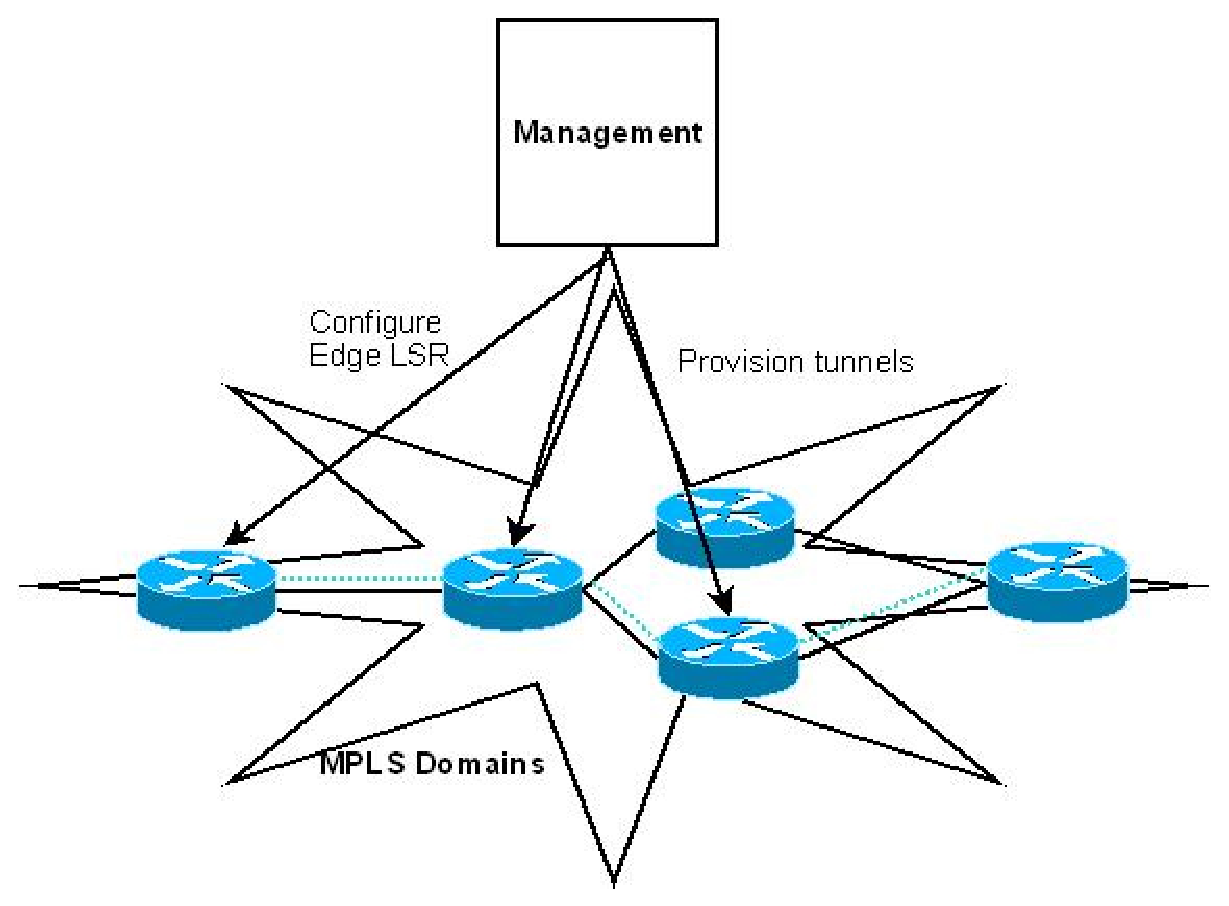
\epsfig{file=img/sec-2-1/TE2, width=4.5in}
\caption{
   Configuration of tunnels and control admission in MPLS networks.
    \label{fig:mpls-header}
}
\end{center}
\end{figure}


\subsection{Limitations}
	In both Traffic Engineering approaches, IP based and CBR in MPLS, the optimization of the routing is carried out for an estimation of the future demand based on long term measurement of the current traffic and expectation of evolution.  This is why both mechanisms are referred to as offline solution and raises some limitations. Indeed, actual traffic might differ from the network estimation and hence the routing might result in suboptimal or even inadequate distribution of the traffic on the network. Attacks, changes on external routing and link failures are frequent events and affect the traffic demands on the network. Failures are particularly wake point for this approach of routing. Offline TE deals with network failures by pre-computing alternatives routes. However, this could be done only for a limited set of network failures and TE should look for reroutes that perform relatively for a range of failures. As a result, suboptimal utilization of the network is frequent. Online TE is necessary to ensure that the network adapts in real time to changes on the demand.
	
A second characteristic of the previous approaches is that they require a global vision of the network to choose the configuration parameters. Some constraints are related to this property, like the scalability of the solution and the frequency of the update of the parameters. In distributive schemes, most of the decisions are made locally without requiring frequent interventions from a  central entity. 
In the next section, an example of a new TE solution that mitigates some of the limitation described above.

\subsection{Example of an adaptive traffic engineering protocol: TEXCP }

TEXCP is a dynamic and distributed TE protocol that targets the optimization of network utilization. The basic idea behind TEXCP is that using path diversity we could balance the load among available paths in a way that optimizes utilization performance within a network. It is not itself a routing protocol but it sets on the top of existing MPLS systems and control how the flows are distributed over the network.

TEXCP is an online mechanism, meaning that it reacts to the changes on the traffic demands and potential network failures. It is distributed and doesn't necessitate an oracle that has a global vision of the network, boosting though its capability to scale in large networks. But, most importantly TEXCP has proved a strong stability that lacked most of the dynamic TE solutions until now. 
It targets performance optimization within a single domain, though it is considered as an Inter-Domain TE method. To have a more concrete idea, let's consider the simple architecture in (\ref{fig:texcp1}) :
\begin{figure}[h]
 \begin{center}

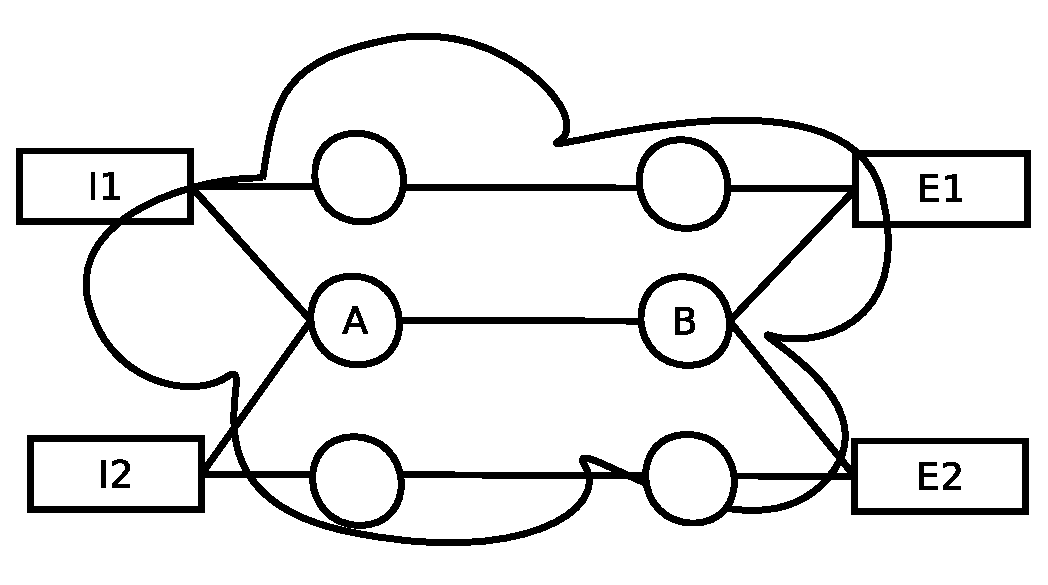
\epsfig{file=img/sec-2-1/TEXCPArchitecture, width=4.5in}
\caption{
   A simple architecture of an ISP network.
    \label{fig:texcp1}
}
\end{center}
\end{figure}
\\ From the ISP perspective, a flow enter the domain in an Ingress point (For instance I1) and leaves it in an egress point (E1 for instance). For this Ingress/Egress IE pair, two paths are available. In MPLS, as we've seen in the previous section, every packet arriving at the  domain will have a label allocated with the path it should takes. The path is chosen to meet a load balancing target: this load balancer called an agent will be associated to each IE pair and has as a target to balance the traffic among the preselected paths. The agent is also responsible of continuously probing the state of the network to feed the balancer with path utilization info. The probing mechanism is also used by the core routers to prevent oscillation and control the congestion.

{\bf Probing Network State}
\\ TEXCP load balancer needs to keep a track of the utilization state for each of the available paths. Hence the agent has to send a probe over all the available paths of  the IE pair associated to.  This probe will be processed by every router on the path until reaching the egress point, that will send back an acknowledgement message directly to the ingress. The format of the probe is shown in figure \ref{fig:texcp2}
\begin{figure}[h]
 \begin{center}
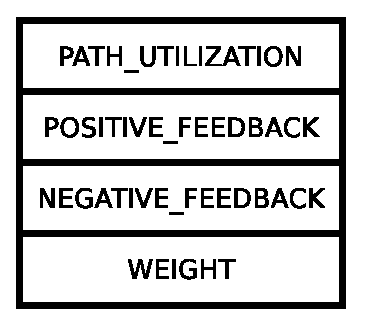
\epsfig{file=img/sec-2-1/TEXCPProbe, width=2in}
\caption{
   A simple architecture of an ISP network.
    \label{fig:texcp2}
}
\end{center}
\end{figure}
\\ The separation interval $T_p$ between two consecutive probes should be larger than the maximum round trip time RTT. However, the smaller is this value the faster the algorithm will converge. And hence it should be chosen slightly larger than RTT. A typical value for an average network is 100ms. During network congestion periods, it is possible that the probe get lost.

{\bf The Load balancer}
\\ As mentioned previously, TEXCP objective is minimizing the utilization in the network. Let's try to put this problem in a more formal way. Let $s$ an IE pair, and $P_s$ the set of selected paths for pair $s$. If $x_{sp}$ denotes the positive fraction of IE pair s traffic that goes through path p, the load balancer problem is to find the $(x_sp)$ configuration that will minimize the maximum utilization over all the network links 
\begin{equation}
\min_{x_{sp}} max_{l \in L} u_{l}
\end{equation}
subject to the following conditions:
\begin{equation}
u_l = \sum_{s} \sum_{p \in P / l \in p} \frac {x_{sp} }{C_l}
\end{equation}
\begin{equation}
\sum_{p \in P_{s}} x_{sp} = 1,  \forall s
\end{equation}
\\ This could be achieved if every agent tried to equalize the loss that it sees over all the controlled paths. According to the path utilization and the current rate distribution, the agent will send more traffic on underutilized paths and less traffic on over-utilized ones. This amount is calculated according to:
\begin{equation}
\Delta x_{sp} = \frac{r_{sp}} {\sum r_{sp'}}  (u' - u_{sp}) 
\end{equation}
Where $u'$ the average path utilization. For the path with the minimum utilization a small positive factor is added to avoid that the oath with current small rate stop being used. The new value is path ratio could be calculated as the equation bellow then normalized:
\begin{equation}
x_{sp} = max(0, x_{sp} + \Delta x_{sp}
\end{equation}

{\bf Feedback}
\\Due to the distributed nature of TEXCP, instability and oscillation may occur. Let's consider again the simplified architecture in figure \ref{fig:texcp1}. Link AB, is shared between pair I1E1 and pair I2E2 and hence in the case where the link is underutilized, agents associated with both pair will react by sending more traffic over this link and potentially causing the link to be over-utilized. Hence, it is necessary to have a feedback mechanism that will allow the core nodes -in particular node A-  to control and synchronize the answer of the multiple TEXCP agents that use the link. This mechanism is similar to what is used for congestion control when multiple sources sharing the same bottleneck attempts to adjust their rate and end up causing the bottleneck utilization to oscillate. The solution for both problems is to explicitly inform the sources of how much they should increase or decrease their rate. In order to provide the sources with such information, every core router needs first to update the aggregate feedback every $T_{p}$ seconds and then include within the probe. The aggregate feedback is an upper bound of how much the global traffic sent to the link should increase/decrease. Hence, the aggregate feedback is positively proportional to the spare bandwidth S (S = capacity -load) over the link and the negatively to the current buffer size Q.
\begin {equation}
\phi = \alpha . T_{p} . S - \beta . Q
\end {equation}
The next step is to divide this aggregate feedback over the available sources, TEXCP adopt a Max-Min allocation policy to divide this aggregate feedback, and hence installing a fairness that will prevent congested IE pairs from starving the others. Additive Increase Multiplicative Decrease (AIMD) standard is used to achieve this fairness and hence: 
\begin {eqnarray}
\Phi \ge 0 \Rightarrow \delta^+ = \frac{\Phi} {N}, \delta^- = 0 \\
\Phi \ge 0 \Rightarrow \delta^+ = 0 , \delta^- = \frac{\Phi} \phi_l
\end {eqnarray}
Where N denotes the number of active IE pairs that the router is seeing, and $\phi_l$ is the aggregate load on link l.

Before continuing on how this information is sent back to the IE agents, we would like to turn the reader attention to the scenario where multiple solutions of the optimization problem exist: consider a simple example where the two IE pairs in figure ?? have the same traffic, and that the two links have the same capacity. One solution is that each router send one half of its traffic over each link, while the second solution is that the first pair send all its traffic in link 1 while the other pair use the other link. In both solution the network utilization is the same and optimal, however the second solution has the merit of a reduce delay. So it we be good in case where multiple solution exist, shortest path are prioritized. This condition could be implement through the use of a weighted fairness allocation of the aggregate feedback 
When the ingress router send the probe, the fields will be updated by each router as:\\
\begin{eqnarray}
PATH-UTILIZATION = max (PATH-UTILIZATION, ul ) \\
POSITIVE-FEEDBACK = min (POSITIVE-FEEDBACK, \delta^+ ) \\
NEGATIVE-FEEDBACK = max (NEGATIVE-FEEDBACK, \delta^− ) 
\end{eqnarray}
Once the probe reaches the egress router, the router sends back directly the final values. The first field in the probe is the utilization of the most congested path and in a similar way, the value for the feedback. The agent will update his sending rate $g_sp$ according to AIMD:
\begin{equation}
g_{sp} = g_{sp} + \delta^+ - g_{sp} \cdot \delta^-.
\end{equation}

\subsection{Splitting the traffic : FLARE}

\\ What the agent needs to do is to update $(x_{sp})$ the splitting ratio of the incoming traffic over the available paths. Traditionally, traffic splitting was tackled from two approaches. The first one is packet-based. However, this solution is very harmful to transport protocols that are sensitive to packet reordering like TCP. The second solution to split in flow basis, i.e. all packet of the same flows are sent over the same path. By assuring that a flow's packets goes over the same path, packet reordering won't take place and hence TCP could achieve a better performance. However, the flows have different sizes and characteristics hence this approach of traffic splitting deviates usually from the desired splitting ratio. An intermediate solution is described in \cite {sin1}, that take advantage from TCP burtsiness to do the splitting. A TCP flow life cycle is divided into a set of packets bursts called flowlet separated by idle periods. The flow-lets could be characterized by the minimum time that separate two successive flowlets. If we rightly choose this value larger then the value of delay difference, we could send the packets of the different flowlets in different paths without risking reordering problems: Let's consider a simple scenario where the last packet of a flowlet leaves the paths divergence points at time $t_0$. If we know that the when the 
FLARE suggest also a splitting mechanism that uses a Token-counting algorithm, 
The final algorithm could be sum up in the following 3 steps:

1-when a packet arrives the counters of all the flows are updated as follows:
\begin{equation}
c_{sp} = c{sp} + x_{sp} \cdot PacketSize.
\end{equation}

2- if the packet flow is not TCP or the last time the flow has been seen is older then the time out value, the packet is sent on a the path with the highest token counter value. The packet is sent over the same path as the last packet of the flowlet.\\

3-The last seen time is updated as well as the counter of the selected path according to :
\begin{equation}
c_{sp} = c{sp} - PacketSize.
\end{equation}
